%%
%% CSE 333/533 - Assignment 02: Transformations, Viewing and Projection
%% Author: Keshav Singh (Roll No. 2024300)
%%
\documentclass[acmlarge]{acmart}

\usepackage{amsmath}
\usepackage{listings}
\usepackage{xcolor}
\usepackage{cleveref}   % after hyperref (loaded by acmart)

\lstset{
  language=C++,
  basicstyle=\footnotesize\ttfamily,
  keywordstyle=\color{blue},
  commentstyle=\color{gray},
  numbers=none,
  frame=single,
  breaklines=true,
  showstringspaces=false
}

\emergencystretch=2em

\begin{document}

\title{Assignment 02: Transformations, Viewing, and Projection}

\author{Keshav Singh}
\email{keshav24300@iiitd.ac.in}
\affiliation{%
  \institution{Indraprastha Institute of Information Technology, Delhi}
  \city{New Delhi}
  \country{India}
}

\begin{abstract}
This report describes camera motion along a 3D spiral for Assignment~02 of
CSE~333/533. The camera rides on the spiral and looks at the origin, with
perspective and orthographic projection, pause/resume and manual stepping. We
derive the tangent vector analytically, build an orthonormal camera basis from
it, and prove that this basis is never degenerate for the given spiral.
\end{abstract}

\keywords{spiral camera motion, viewing transformation, projection,
orthonormal basis, OpenGL}

\maketitle
\newpage

\section{Notation and Design}

The camera moves along the spiral
\begin{align}
  x(\theta) &= r(\theta)\cos(k\theta), \label{eq:x}\\
  y(\theta) &= h\cos\theta, \label{eq:y}\\
  z(\theta) &= r(\theta)\sin(k\theta), \label{eq:z}
\end{align}
with $r(\theta)=\sqrt{R^2+4h^2\cos^2\theta}$, neck radius $R$, height $2h$,
$k$ cycles and $\theta\in[0,2\pi]$; the program uses $R=h=25$, $k=8$. The program builds on the template code provided by the course teaching staff~\cite{template}, written in C++ with OpenGL~\cite{khronos}, GLFW~\cite{glfw} for the window and keyboard input, Dear ImGui~\cite{imgui} for the interface and GLM~\cite{glm} for the view and projection matrices; the viewing and projection pipeline follows~\cite{learnopengl}.

\paragraph{Design choices.} The camera state is only the scalar
\texttt{spiralTheta} plus the flags \texttt{isPaused}, \texttt{isOrthographic}
and \texttt{isq1}. The camera position and frame are recomputed from
\texttt{spiralTheta} at every update, so no history is stored. Keys
\texttt{1}/\texttt{2} select the Q1 camera (fixed $Y$ up) or the Q2 camera
(tangent-based frame).

\section{Task 1}

\subsection{Camera on the spiral (Q1a)}

\texttt{spiral()} evaluates \cref{eq:x,eq:y,eq:z} at \texttt{spiralTheta} to
give the camera position $\mathbf{C}$, and
\begin{lstlisting}
view = glm::lookAt(camPos, glm::vec3(0.0), glm::vec3(0.0, 1.0, 0.0));
\end{lstlisting}
looks at the origin with $Y$ up. This is always valid: $\|\mathbf{C}\|\ge
r(\theta)\ge R>0$ and $\mathbf{C}$ has a nonzero horizontal part, so it is never
parallel to the up vector. A frame is shown in \cref{fig:q1}(a).

\subsection{Projection toggle (Q1b)}

\texttt{O} sets \texttt{isOrthographic = true} and \texttt{P} sets it to false;
the projection matrix is rebuilt immediately after each change. A frame is shown
in \cref{fig:q1}(b).

\begin{figure}[t]
  \centering
  \begin{minipage}[t]{0.48\linewidth}
    \centering
    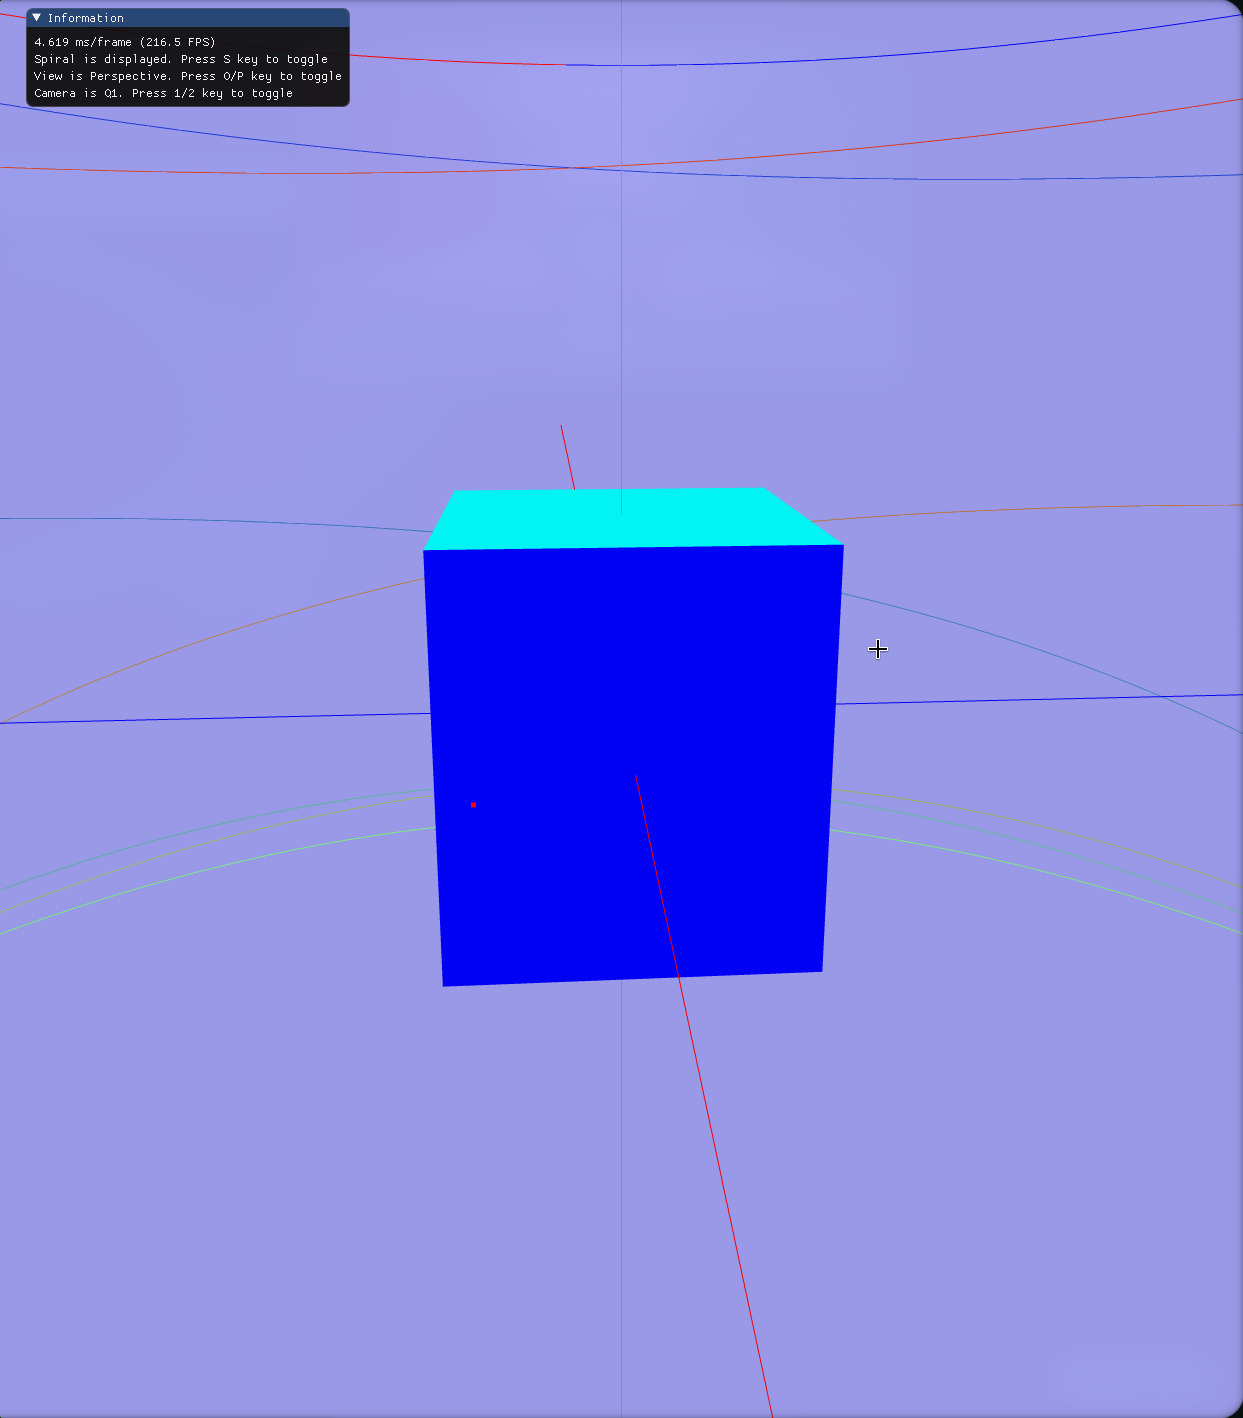
\includegraphics[width=\linewidth,height=0.3\textheight,keepaspectratio]{1}\\
    (a) Perspective (Q1a)
  \end{minipage}\hfill
  \begin{minipage}[t]{0.48\linewidth}
    \centering
    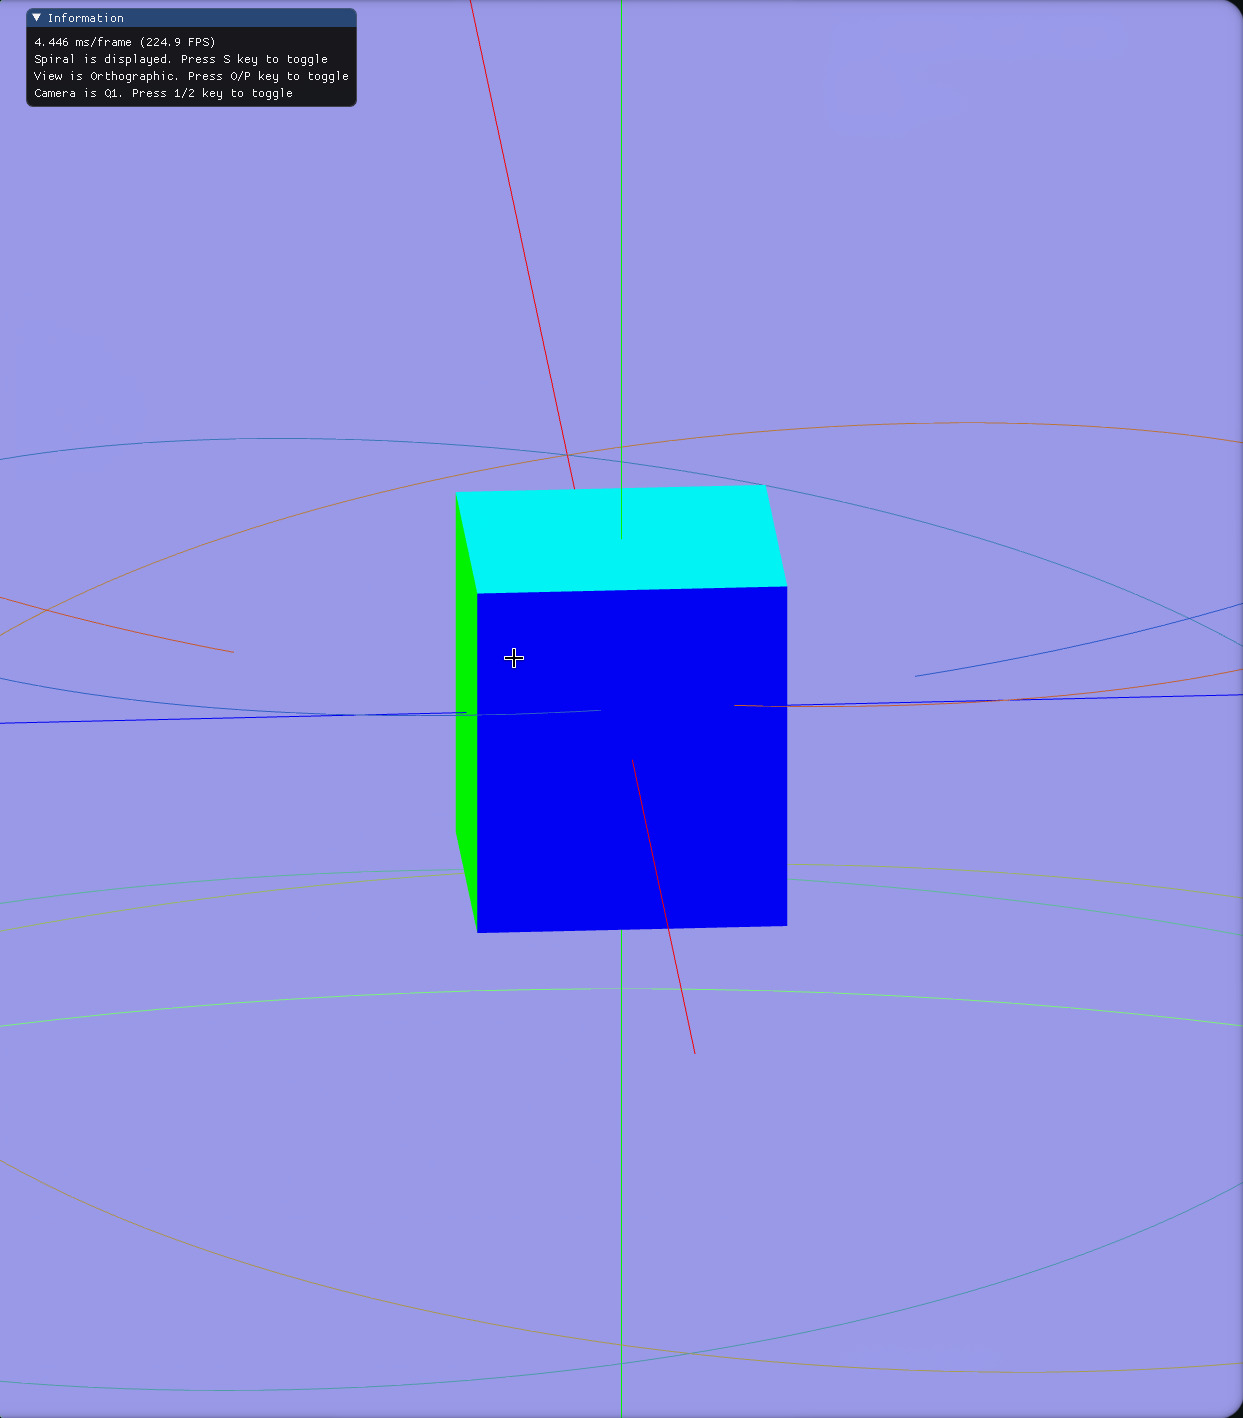
\includegraphics[width=\linewidth,height=0.3\textheight,keepaspectratio]{2}\\
    (b) Orthographic (Q1b)
  \end{minipage}
  \caption{Camera on the spiral looking at the origin with $Y$ up.}
  \Description{Two screenshots of the cube and spiral seen from a camera on the
  spiral: left in perspective projection, right in orthographic projection.}
  \label{fig:q1}
\end{figure}

\subsection{Pause/resume and manual stepping (Q1c)}

Space toggles \texttt{isPaused}; on resume the accumulator is cleared so the
animation does not jump. While paused, Left/Right decrease/increase
\texttt{spiralTheta} by half an animation step ($0.125^\circ$) and update the
view immediately. No wrapping is needed for manual steps since the curve is
periodic.
\begin{lstlisting}
if (!io.WantCaptureKeyboard && ImGui::IsKeyPressed(GLFW_KEY_SPACE)) {
  isPaused = !isPaused;
  if (!isPaused) timeAccumulator = 0;
}
if (!io.WantCaptureKeyboard && ImGui::IsKeyPressed(GLFW_KEY_LEFT) && isPaused) {
  spiralTheta -= spiralDeltaTheta * 0.5;
  setupViewTransformation(shaderProgram, spiralTheta);
}
if (!io.WantCaptureKeyboard && ImGui::IsKeyPressed(GLFW_KEY_RIGHT) && isPaused) {
  spiralTheta += spiralDeltaTheta * 0.5;
  setupViewTransformation(shaderProgram, spiralTheta);
}

float dt = ImGui::GetIO().DeltaTime;
timeAccumulator += dt;
if (timeAccumulator >= updateInterval && !isPaused) {
  timeAccumulator -= updateInterval;
  spiralTheta += spiralDeltaTheta;
  if (spiralTheta >= 2.0 * M_PI) spiralTheta -= 2.0 * M_PI;
  setupViewTransformation(shaderProgram, spiralTheta);
}
\end{lstlisting}

\begin{center}
\begin{tabular}{@{}ll@{}}
\texttt{O} / \texttt{P} & orthographic / perspective projection\\
\texttt{Space} & pause / resume\\
\texttt{Left} / \texttt{Right} & decrease / increase \texttt{spiralTheta} (paused)\\
\texttt{1} / \texttt{2} & Q1 camera / Q2 camera\\
\end{tabular}
\end{center}

\section{Task 2}

\subsection{Tangent vector (Q2a)}

We denote the tangent $\mathbf{v}(\theta)$ of the assignment by $\mathbf{t}(\theta)$,
to keep $\mathbf{v}$ free for the camera basis below. From \cref{eq:y},
$dy/d\theta=-h\sin\theta$. Differentiating $r^2=R^2+4h^2\cos^2\theta$ gives
\begin{equation}
  r'(\theta)=-\frac{4h^2\cos\theta\sin\theta}{r(\theta)}.
\end{equation}
By the product rule,
\begin{align}
  \frac{dx}{d\theta}&=r'\cos k\theta-k\,r\sin k\theta,\\
  \frac{dz}{d\theta}&=r'\sin k\theta+k\,r\cos k\theta.
\end{align}
With $\mathbf{e}_r=(\cos k\theta,0,\sin k\theta)$,
$\mathbf{e}_\phi=(-\sin k\theta,0,\cos k\theta)$, $\mathbf{e}_y=(0,1,0)$,
\begin{equation}
  \mathbf{t}(\theta)=r'\,\mathbf{e}_r+k\,r\,\mathbf{e}_\phi-h\sin\theta\,\mathbf{e}_y .
  \label{eq:t}
\end{equation}
Since $kr\ge kR>0$, $\mathbf{t}\neq\mathbf{0}$ for every $\theta$. The program
evaluates this in \texttt{spiral\_derivative()}.

\subsection{Orthonormal camera basis (Q2b)}

Let $\mathbf{C}(\theta)$ be the camera position, $\mathbf{g}=-\mathbf{C}$ the gaze
vector and $\mathbf{y}=(0,1,0)$. We build the basis $(\mathbf{u},\mathbf{v},\mathbf{w})$
(camera right, up and backward axes) as follows.
\begin{enumerate}
  \item $\mathbf{w}=-\mathbf{g}/\|\mathbf{g}\|=\mathbf{C}/\|\mathbf{C}\|$.
  \item $\mathbf{u}$ must lie in the plane of $\mathbf{g}$ and $\mathbf{t}$ and be
  perpendicular to $\mathbf{w}$, so $\mathbf{u}=\pm\mathbf{t}_\perp/\|\mathbf{t}_\perp\|$
  with $\mathbf{t}_\perp=\mathbf{t}-(\mathbf{t}\cdot\mathbf{w})\mathbf{w}$.
  \item $\mathbf{v}=\mathbf{w}\times\mathbf{u}$ is then perpendicular to that plane,
  i.e.\ $\mathbf{v}=\pm\mathbf{n}/\|\mathbf{n}\|$ with
  $\mathbf{n}=\mathbf{t}\times\mathbf{C}$. The two signs are the only freedom left,
  and ``$\mathbf{v}$ as close as possible to $\mathbf{y}$'' selects the one with
  $\mathbf{v}\cdot\mathbf{y}>0$.
\end{enumerate}
Hence $\mathbf{v}=\mathbf{n}/\|\mathbf{n}\|$ (shown below to have $\mathbf{v}\cdot\mathbf{y}>0$
always) and $\mathbf{u}=\mathbf{v}\times\mathbf{w}=-\mathbf{t}_\perp/\|\mathbf{t}_\perp\|$.
In code, \texttt{updir = cross(-camPos, t)} $=\mathbf{n}$ is passed to
\texttt{glm::lookAt(camPos, origin, updir)}, which builds exactly this frame (its
right vector is $\mathbf{u}$ and its backward axis is $\mathbf{w}$). The schematic
is in \cref{fig:frame}.

\begin{figure}[t]
  \centering
  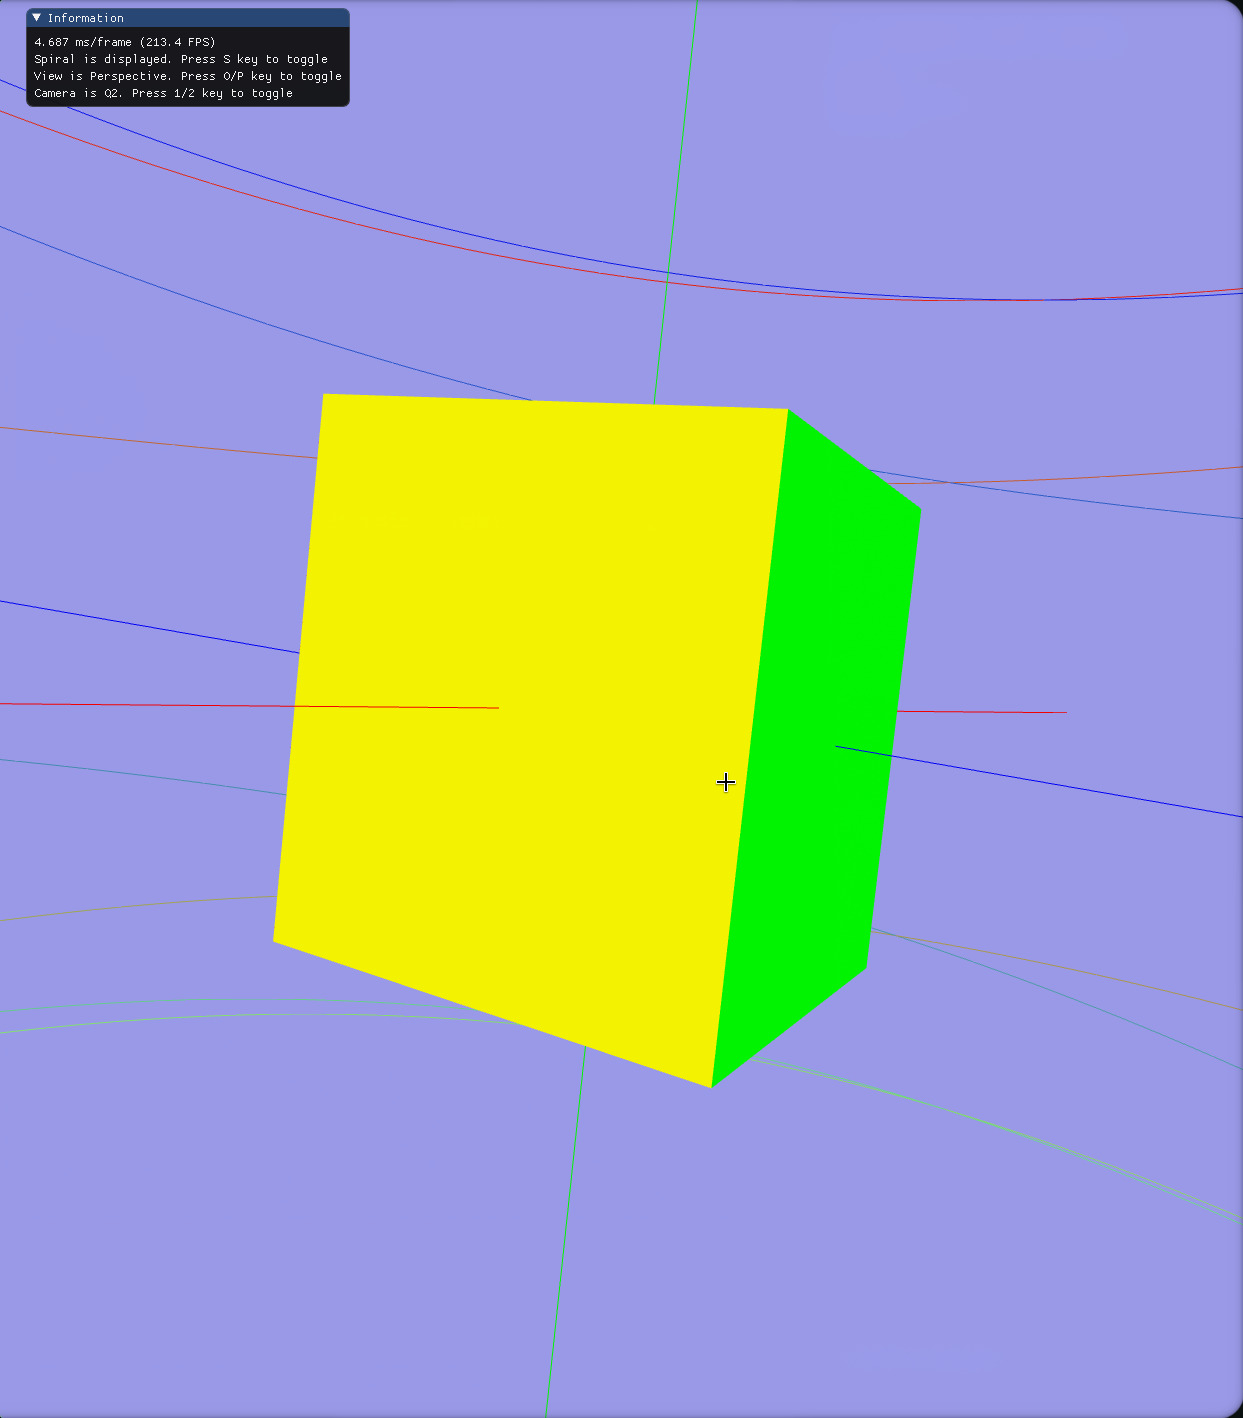
\includegraphics[width=0.6\linewidth,height=0.35\textheight,keepaspectratio]{3}
  \caption{Camera coordinate frame relative to the world frame and a small part
  of the spiral around the camera.}
  \Description{Hand-drawn sketch of the camera axes u, v, w at a point on the spiral, relative to the world axes.}
  \label{fig:frame}
\end{figure}

\begin{proposition}\label{prop:nondeg}
For $R>0$ and integer $k\ge1$, $\mathbf{n}=\mathbf{t}\times\mathbf{C}$ is nonzero
for every $\theta$, $\{\mathbf{u},\mathbf{v},\mathbf{w}\}$ is an orthonormal basis,
and $\mathbf{v}\cdot\mathbf{y}>0$.
\end{proposition}

\begin{proof}
Write $\mathbf{C}=r\,\mathbf{e}_r+y\,\mathbf{e}_y$ with $y=h\cos\theta$, and
use \cref{eq:t} with $y'=-h\sin\theta$. The cross products of the cylindrical
basis are $\mathbf{e}_r\times\mathbf{e}_\phi=-\mathbf{e}_y$,
$\mathbf{e}_r\times\mathbf{e}_y=\mathbf{e}_\phi$ and
$\mathbf{e}_y\times\mathbf{e}_\phi=\mathbf{e}_r$. Expanding,
\begin{equation}
  \mathbf{n}=-k\,r\,y\;\mathbf{e}_r-(r\,y'-y\,r')\,\mathbf{e}_\phi+k\,r^2\,\mathbf{e}_y .
  \label{eq:n}
\end{equation}
The $\mathbf{e}_y$ component is $kr^2\ge kR^2>0$, so $\|\mathbf{n}\|\ge kR^2>0$
for all $\theta$; hence $\mathbf{C}$ and $\mathbf{t}$ are never parallel and
$\mathbf{t}_\perp\neq\mathbf{0}$. Since $\mathbf{n}\perp\mathbf{C}$ and
$\mathbf{n}\perp\mathbf{t}$, $\mathbf{v}=\mathbf{n}/\|\mathbf{n}\|$ is a unit
vector orthogonal to $\mathbf{w}$ and $\mathbf{u}$, and $\mathbf{u}=\mathbf{v}\times\mathbf{w}$
completes a right-handed orthonormal basis. Finally
$\mathbf{v}\cdot\mathbf{y}=kr^2/\|\mathbf{n}\|>0$.
\end{proof}

\subsection{Smoothness (Q2c)}

By \cref{eq:n}, $\mathbf{n}$ is a smooth, $2\pi$-periodic function of $\theta$
that never vanishes, so $\mathbf{v}$, $\mathbf{w}$ and $\mathbf{u}$ vary
continuously, including at the loop closure $\theta=2\pi\to0$. Because
$\mathbf{v}\cdot\mathbf{y}>0$ for every $\theta$, the sign choice is the same
everywhere and the camera stays upright, so no flipping is needed or performed.
The animation is therefore smooth. The remaining visible effect is fast rotation
about the $Y$ axis, since the camera makes $k$ turns around it per period, and
the image is rolled relative to Task~1 because $\mathbf{v}$ is tied to the
tangent rather than to $\mathbf{y}$.

\paragraph{Issue encountered.} An earlier version of our code chose the sign of
the up vector by testing the $Y$ component of the camera's right vector, negating
the up vector when it was positive. From \cref{eq:n}, that component is
$u_y=hR^2\sin\theta/(\|\mathbf{C}\|\|\mathbf{n}\|)$, which changes sign at
$\theta=0$ and $\theta=\pi$. The test therefore reversed the up vector at these
two points: a $180^\circ$ roll jump twice per loop (numerically $179.9^\circ$
between samples $0.02^\circ$ apart, versus an average of $0.88^\circ$ between
consecutive frames), with the camera upside-down for $\theta\in(0,\pi)$. The
camera basis itself was never degenerate; only the sign normalisation was at
fault. Testing $\mathbf{v}\cdot\mathbf{y}$ instead, or equivalently dropping the
test (it never triggers by Proposition~\ref{prop:nondeg}), removes the problem.

\section{Animations}

The recordings of the three animations (perspective, orthographic, and the
tangent-based camera of Task~2) are included as \texttt{.mp4} files in the code
folder of the submission.


\begin{thebibliography}{6}

\bibitem[LearnOpenGL]{learnopengl}
\emph{LearnOpenGL Shaders}.
\newblock Accessed via \url{https://learnopengl.com/Getting-started/Shaders}.

\bibitem[OpenGL]{opengldoc}
OpenGL: \emph{Official Documentation}.
\newblock Accessed via \url{https://www.opengl.org/documentation/}.

\bibitem[Khronos]{khronosgl}
Khronos OpenGL Wiki: \emph{Rendering Pipeline Overview}.
\newblock Accessed via \url{https://www.khronos.org/opengl/wiki/Rendering_Pipeline_Overview}.

\bibitem[GLFW]{glfwdoc}
GLFW: \emph{Documentation}.
\newblock Accessed via \url{https://www.glfw.org/documentation.html}.

\bibitem[docs.gl]{docsgl}
docs.gl: \emph{OpenGL API Reference}.
\newblock Accessed via \url{https://docs.gl}.

\end{thebibliography}

\end{document}
